\documentclass{beamer}
\usepackage{amsfonts,amsmath}
\usetheme{-statale}
\usefonttheme[onlymath]{serif}

\usepackage[italian]{babel}
\usepackage{bussproofs}
\usepackage{tabularx}
\usepackage{multirow}
\usepackage{tabularray}
\usepackage[makeroom, thicklines]{cancel}

\usepackage{float}
\usepackage{subcaption}
\usepackage{tikz}
\usetikzlibrary{positioning}
\usepackage{stmaryrd}
\usepackage{subcaption}
\usepackage{caption}
\usepackage{siunitx}

\EnableBpAbbreviations

\newcommand{\testcolor}[1]{\colorbox{#1}{\textcolor{#1}{test}}~\texttt{#1}}
\newcommand{\hrefcol}[2]{\textcolor{cyan}{\href{#1}{#2}}}

\definecolor{lightbluestatale}{RGB}{34, 167, 229}
\definecolor{darkbluestatale}{RGB}{0, 51, 102}

\newcommand{\llpar}{\rotatebox[origin=c]{180}{$\&$}}
\newcommand{\llten}{\otimes}
\newcommand{\llwith}{\&}
\newcommand{\llplus}{\oplus}
\newcommand{\llbot}{\bot}
\newcommand{\lltop}{\top}
\newcommand{\llone}{1}
\newcommand{\llzero}{0}

\titlebackground*{images/theme/background}

\title{Proof Search in Propositional Linear Logic via Boolean Constraints Satisfaction}
\course{Laurea Triennale in Informatica}
\author{Martino D'Adda}
\IDnumber{964827}

\begin{document}

\maketitle

\footlinecolor{maincolor}

\section{Introduzione}
\begin{frame}{Calcolo dei sequenti}
	Il calcolo dei sequenti  è un sistema formale  introdotto da G.Gentzen nel 1935 che può essere usato per specificare la ricerca di prove (\textit{proof search}) in logica, basato su:
	\begin{itemize}
		\item<2-> il sequente $\Delta \vdash \Gamma$, di solito interpretato come
			$$ \delta_1 \wedge \dots \wedge \delta_n \rightarrow \gamma_1 \vee \dots \vee \gamma_m $$
		\item<3-> la regola, che descrive come manipolare i sequenti
			\begin{itemize}
				\item descrive la semantica di un connettivo (introduzione e eliminazione):
					\vspace*{.1cm}
					\begin{center}
						\begin{tabular}{cc}
							$$
							\AXC{$\Delta \vdash \phi', \Gamma$}
							\AXC{$\Delta \vdash \phi'', \Gamma$}
							\LeftLabel{$\text{intro} \wedge$}
							\BIC{$\Delta \vdash \phi' \wedge \phi'', \Gamma$}
							\DP
							$$
							&
							$$
							\AXC{$\Delta, \phi', \phi'' \vdash \Gamma$}
							\LeftLabel{$\text{elim} \wedge$}
							\UIC{$\Delta, \phi' \wedge \phi'' \vdash \Gamma$}
							\DP
							$$
						\end{tabular}
					\end{center}
					\vspace*{.1cm}
				\item descrive come trattare le formule all'interno del sequente (regole strutturali).
			\end{itemize}
		\item<4-> la dimostrazione, un albero avente come radice il sequente da dimostrare e ottenuto concatenando regole.
	\end{itemize}
\end{frame}

\begin{frame}{Proof search}
	Un \textbf{theorem prover} è un programma che, dato un sequente, prova a costruirne la dimostrazione.
	Nello specifico nella versione bottom-up:
	\begin{enumerate}
		\item si sceglie un \textit{goal}, inizialmente il sequente iniziale;
		\item lo si scompone applicando una regola ad una delle formule nel goal;
		\item si aggiungono i nuovi goal al working-set;
		\item si ripete dal passo 1 fino a che ci sono goal irrisolti.
	\end{enumerate}
\end{frame}

\begin{frame}{Focusing}
	Nella maggior parte dei casi ci saranno più regole applicabili ad un sequente, ma non tutte le scelte sono uguali:
	\begin{itemize}
		\item certe sono \textit{invertibili} e possono essere applicate in qualunque ordine senza perdere completezza (non-determinismo don't-care),
		\item altre richiedono scelte e creano punti di backtracking (non-determinismo don't-know).
	\end{itemize}
	Il \textbf{focusing} è una tecnica che suddivide la dimostrazione in due fasi che si alternano:
	\begin{itemize}
		\item asincrona: si applicano eagerly solo regole invertibili (non-determinismo don't-care);
		\item sincrona: ci si concentra su una formula e si continuano ad applicare regole non invertibili (non-determinismo don't-know).
	\end{itemize}
\end{frame}

\begin{frame}{Logica lineare}
	La \textbf{logica lineare} nasce dall'analisi delle regole strutturali e dall'abbandono di due di esse:
	\begin{itemize}
		\item \textit{weakening}: nel sequente si possono sempre aggiungere formule;
		\item \textit{contraction}: due copie della stessa formula possono essere contratte.
	\end{itemize}
	Nella logica che ne risulta:
	\begin{itemize}
        	\item ogni formula deve essere usata esattamente una volta;
        	\item le formule possono essere viste come \textbf{risorse};
		\item ogni connettivo ammette due versioni, una additiva ed una moltiplicativa, corrispondenti a due diverse interpretazioni dei connettivi classici;
	\end{itemize}
	Degli speciali connettivi, chiamati esponenziali, permettono di localizzare weakening e contrazione.
\end{frame}

\begin{frame}{Gestione delle risorse}
	Durante il proof searching bottom-up in logica lineare un'ulteriore fonte di non-determinismo è la gestione delle risorse.
	$$
	\AXC{}
	\LeftLabel{$A$}
	\UIC{$\phi' \vdash \phi'' $}
	\AXC{}
	\LeftLabel{$A$}
	\UIC{$\phi' \vdash \phi'' $}
	\LeftLabel{$\llten_R$}
	\BIC{$\phi', \phi'' \vdash \phi'' \llten \phi' $}
	\LeftLabel{$\llten_L$}
	\UIC{$\phi' \llten \phi'' \vdash \phi' \llten \phi''$}
	\DP
	$$

        Le regole moltiplicative richiedono di scegliere un partizionamento corretto del contesto (\textbf{splitting}), operazione potenzialmente esponenziale.
        
\end{frame}
\section{Il nostro calcolo}
\begin{frame}{Calcolo dei vincoli}
	Nel 2001 D.Pym e J.Harland propongono una gestione delle risorse basato su \textbf{vincoli booleani}.
	Questi
	\begin{itemize}
		\item generati durante la proof-search a partire da espressioni associate alle formule;
		\item  due tipi:
			\begin{itemize}
				\item una certa formula è stata usata nel goal corrente, e non può essere usata altrove;
				\item una certa formula non è stata usata, ed è disponibile altrove;
			\end{itemize}
	\end{itemize}
	La soddisfacibilità del vincolo rimpiazza lo splitting del   contesto
	$$
	\AXC{}
	\LeftLabel{$A$}
	\UIC{$\cancel{\phi'}, \phi'' \vdash \phi'' $}
	\AXC{}
	\LeftLabel{$A$}
	\UIC{$\phi', \cancel{\phi''} \vdash \phi'$}
	\LeftLabel{$\llten_R$}
	\BIC{$\phi', \phi'' \vdash \phi'' \llten \phi' $}
	\LeftLabel{$\llten_L$}
	\UIC{$\phi' \llten \phi'' \vdash \phi'' \llten \phi' $}
	\DP
	$$
\end{frame}
\begin{frame}{Calcolo dei vincoli cont'd}
	\begin{columns}
		\begin{column}{.6\textwidth}
			Rendiamo il calcolo dei vincoli focused, e di questo nuovo calcolo mostriamo la correttezza esibendo una traduzione tale che il diagramma a lato commuta.
			Con:
			\begin{itemize}
				\item $C$ il nostro calcolo;
				\item $A$ il calcolo focused senza constraint;
				\item $LL$ il calcolo classico della logica lineare.
			\end{itemize}
			e $\llbracket-\rrbracket$ le rispettive traduzioni.
		\end{column}
		\begin{column}{.4\textwidth}
			\begin{center}
				\begin{tikzpicture}[scale=1.5, every node/.style={transform shape}]
					\node (our-calc) {$C$};
					\node (andreoli) [right=of our-calc] {$A$};
					\node (classic)  [below=of andreoli] {$LL$};

					\draw[->] (our-calc) to node[above] {\tiny $\llbracket - \rrbracket_C$} (andreoli);
					\draw[->] (andreoli) to node[right] {\tiny $\llbracket - \rrbracket_A$} (classic);
					\draw[->, dashed] (our-calc) to node[below left] {\tiny $\llbracket - \rrbracket_A \circ \llbracket - \rrbracket_C$} (classic);
				\end{tikzpicture}
			\end{center}
		\end{column}
	\end{columns}
\end{frame}
\begin{frame}{Implementazione}
	Per il nostro calcolo  abbiamo scritto:
	\begin{itemize}
		\item<2-> un'implementazione in SWI-Prolog;
		\item<3-> un generatore di test in OCaml;
		\item<4-> una libreria per il testing e il benchmarking in Python.
	\end{itemize}
	\onslide<5->{Infine l'infrastruttura è stata gestita con Nix.}
	\begin{center}
		\begin{tabular}{*{4}{wc{2cm}}}
			\onslide<2->{
\includegraphics[width=1.5cm]{images/prolog-logo}} &
			\onslide<3->{
\includegraphics[width=1.5cm]{images/ocaml-logo}} &
			\onslide<4->{
\includegraphics[width=1.5cm]{images/python-logo}} &
			\onslide<5->{
\includegraphics[width=1.5cm]{images/nix-logo}} \\
		\end{tabular}
	\end{center}
\end{frame}
\begin{frame}{Prolog}
	Abbiamo scelto SWI-Prolog per:
	\begin{itemize}
		\item la sua capacità di esprimere le regole in modo dichiarativo;
		\item il suo supporto per il backtracking;
		\item le sue librerie per il constraint logic programming (CLP), che offrono una elegante interfaccia verso risolutori di vincoli booleani;
		\item l'unificazione che permette di gestire in automatico la propagazione degli assegnamenti delle variabili booleane.
	\end{itemize}
\end{frame}

\section{Sperimentazione}
\begin{frame}{Risultati}
	\begin{columns}
		\begin{column}{.5\textwidth}
			Il nostro prover è stato confrontato con altri due prover:
			\begin{itemize}
				\item llprover (Prolog, 1997),
				\item APLL (OCaml, 2019).
			\end{itemize}
			Le fonti dei test sono state principalmente due:
			\begin{itemize}
				\item test generati randomicamente (MLL e MALL);
				\item un dataset di traduzioni dalla logica intuizionista per i test esponenziali.
			\end{itemize}
		\end{column}
		\begin{column}{.5\textwidth}
			\begin{figure}[H]
				\centering
				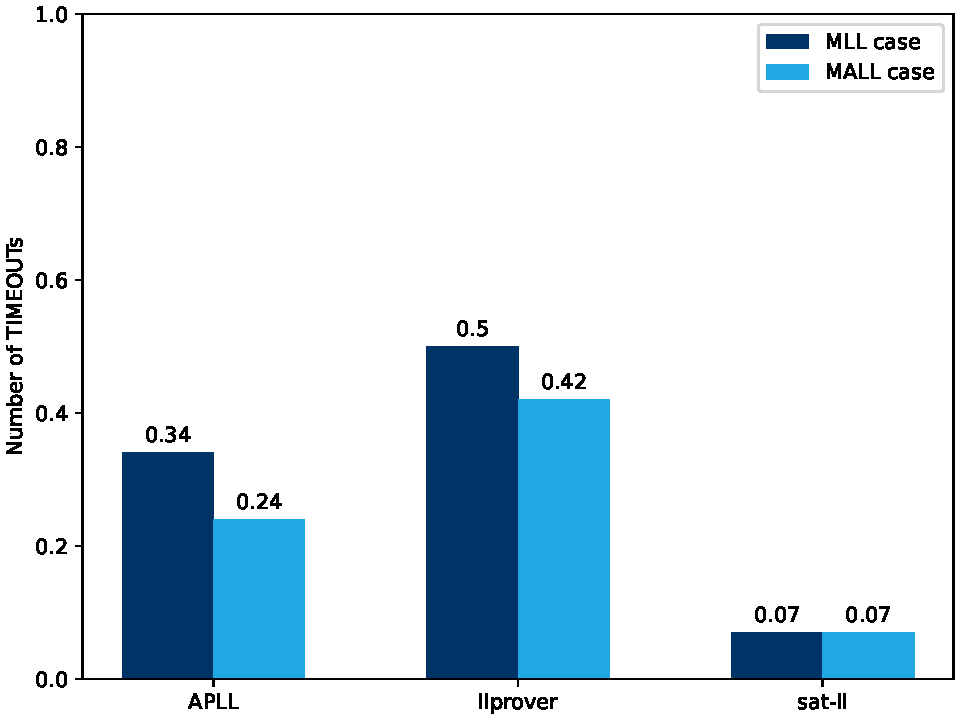
\includegraphics[scale=.4]{images/graph}
			\end{figure}
		\end{column}
	\end{columns}
\end{frame}

\begin{frame}{Conclusione e lavori futuri}
	Del calcolo dei vincoli
	\begin{itemize}
		\item abbiamo fornito un nuovo calcolo che utilizzi il focusing, di cui abbiamo dimostrato la correttezza;
		\item abbiamo fornito un'implementazione in Prolog;
		\item abbiamo confrontato questa implementazione con altri prover simili e mostrato che nel caso moltiplicativo si ottengono buoni risultati.
	\end{itemize}
  	Possibili sviluppi futuri possono essere:
	\begin{itemize}
		\item affinamento dell'algoritmo nel caso esponenziale;
		\item scrittura di altri calcoli e prover simili per altre logiche sotto-strutturali (ILL, BI, ...).
	\end{itemize}
\end{frame}

\backmatter[notitle]
\end{document}
